% -*- mode: fundamental -*-

% ****************************************************************

\chapter{BSV: Rules and Methods II: Improved performance with CRegs (Concurrent Registers)}

\markboth{Ch \arabic{chapter}: BSV: Rules II}{\copyrightnotice}

\setcounter{page}{1}
% \renewcommand{\thepage}{\arabic{page}}
\renewcommand{\thepage}{\arabic{chapter}-\arabic{page}}

\label{ch_Rules_II}

% ****************************************************************

\section{Introduction}

In Section~\ref{Sec_Constraints_on_Mapping_Rules_to_a_Clock} we
discussed constraints on mapping rules into clocked digital hardware.
In particular, executing two rules on the same clock edge may result
in an ordering conflict, and therefore the compiler produces a Rule
Controller to suppress simultaneous firing.  This has some
consequences on the performance of BSV programs, depending on the
primitive modules they use.  We illustrate this problem in
Section~\ref{Sec_Up_Down_Counter}, and then show a general-purpose
solution in Section~\ref{Sec_CRegs} using ``\emph{Concurrent
Registers}'' (or \verb|CReg|s).

Finally, in Section~\ref{Sec_RWires} we show an older solution called
\verb|RWire|s.  We deprecate use of \verb|RWire|s in favor of
\verb|CReg|s, but they are still supported by the compiler (Drum and
Fife codes do not use any \verb|RWire|s).

% ****************************************************************

\section{Example: Counter with {\tt .incr} and {\tt .decr} methods}

\label{Sec_Up_Down_Counter}

Consider the following ``Up-Down Counter'' module interface:

{\footnotesize
\begin{Verbatim}[frame=single, numbers=left]
interface Up_Down_Counter_IFC;
   method Action   incr;
   method Action   decr;
   method Bit #(4) val;
endinterface
\end{Verbatim}
}

The specification for any module implementing this is this:
internally, the module should contain a register that can hold values
in the range 0..15, and, the methods do the following:

\begin{tightlist}
 \item \verb|incr|  increments the counter if it is $< 15$
 \item \verb|decr|  decrements the counter if it is $> 0$
 \item \verb|val|   returns the current value of the counter
\end{tightlist}

Up-down counters are often used for ``credit-based flow control''.
For example, a networking application may send network packets and,
concurrently, receive acknowledgments for previously sent packets, but
the network may not accommodate more than 15 such packets.  Suppose
the register is initialized to 15.  This represents the number of
available ``credits'', {\ie} the number of packets that can be sent
without acknowledgement.  We decrement it whenever a packet is sent,
and increment it whenever an acknowlegement is received.  Thus, it
prevents us from sending more than 15 packets without acknowlegement.

Here is a proposed module to implement the interface:

{\footnotesize
\begin{Verbatim}[frame=single, numbers=left]
module mkUp_Down_Counter_I (Up_Down_Counter_IFC);
   // STATE
   Reg #(Bit #(4)) rg_counter <- mkReg (15);

   // ----------------------------------------------------------------
   // INTERFACE
   method Action incr (rg_counter != 15);
      rg_counter <= rg_counter + 1;
   endmethod

   method Action decr; (rg_counter != 0);
      rg_counter <= rg_counter - 1;
   endmethod

   method Bit #(4) val;
      return rg_counter;
   endmethod
endmodule
\end{Verbatim}
}

% ================================================================

\subsection{Semantic and Performance Analysis of {\tt
            mkUp\_Down\_Counter\_I} when mapped to clocked hardware}

Suppose we have three rules, each invoking one of the three methods on
the same module.  Which pairs of rules can fire on the same clock?

\begin{itemize}

 \item \verb|val| \emph{and} \verb|incr|?

       Yes: Clocked execution is consistent with rule-at-a-time
       semantics where the rule with \verb|val| fires before the rule
       with \verb|incr|.  (And similary, a rule invoking \verb|val|
       can fire on the same clock as a rule invoking \verb|decr|.)

 \item \verb|incr| \emph{and} \verb|decr|?

       No, for both reasons discussed in
       Section~\ref{Sec_Constraints_on_Mapping_Rules_to_a_Clock}.
       There would be an action/resource conflict because both rules
       cannot write the same register at the same instant.  There
       would be an ordering confict because rule-at-a-time semantics
       demands that one rule's update is visible to the other (in
       whichever order they may fire).

\end{itemize}

The key takeaway is that \verb|incr| and \verb|decr| cannot be invoked
on the same clock (same instant).  To revisit our credit-based
flow-control example: on each clock we can either send a packet or
receive an acknowledgement, but not both.

% ****************************************************************

\section{Concurrent Registers {\tt CReg}s, and a Faster Up-Down Counter}

\label{Sec_CRegs}

A Concurrent Register, or \verb|CReg|, is a module provided by the
\emph{bsc} library.  This is an excerpt from the library documentation:

{\footnotesize
\begin{Verbatim}[frame=single, numbers=left]
module mkCReg #(parameter Integer n,
                parameter a_type resetval)
              (Reg#(a_type) ifc[])
\end{Verbatim}
}

The interface is an \emph{array} of register interfaces, indicated by
the square brackets.  A \verb|CReg| module is instantiated with syntax
like this:

{\footnotesize
\begin{Verbatim}[frame=single, numbers=left]
   // parameter n is 2, resetval is 15
   Array #(Reg #(Bit #(4))) crg_counter <- mkCReg (2, 15);
\end{Verbatim}
}

This instantiates a \verb|CReg| whose interface is an array of 2
register interfaces, and whose reset value is 15.  Each interface can
be accessed by indexing: {\tt crg\_counter~[0]} and {\tt
crg\_counter~[1]}.

The key properties of a \verb|CReg| \verb|x| with an array of \verb|n|
register interfaces is:

\begin{itemize}
 \item All the methods can be invoked in the same clock.

 \item A read at the $j$'th register interface,{\ie} {\tt x[$j$].\_read}
       returns the latest of:

       \begin{tightlist}
        \item the value in the register;
        \item if {\tt x[0].\_write($v_0$)} is being invoked, the value $v_0$;
        \item if {\tt x[1].\_write($v_1$)} is being invoked, the value $v_1$;
        \item ...
        \item if {\tt x[$j-1$].\_write($v_{n-1}$)} is being invoked, the value $v_{n-1}$;
       \end{tightlist}

 \item The register value is updated with the latest of:

       \begin{tightlist}
        \item the current value in the register;
        \item if {\tt x[0].\_write($v_0$)} is being invoked, the value $v_0$;
        \item if {\tt x[1].\_write($v_1$)} is being invoked, the value $v_1$;
        \item ...
        \item if {\tt x[$n-1$].\_write($v_{n-1}$)} is being invoked, the value $v_{n-1}$;
       \end{tightlist}
\end{itemize}

% ================================================================

\subsection{A possible hardware implementation of a CReg}

\label{Sec_CReg_HW}

Figure~\ref{Fig_CReg_HW} shows a possible hardware implementation of a CReg.
\begin{figure}[htbp]
  \centerline{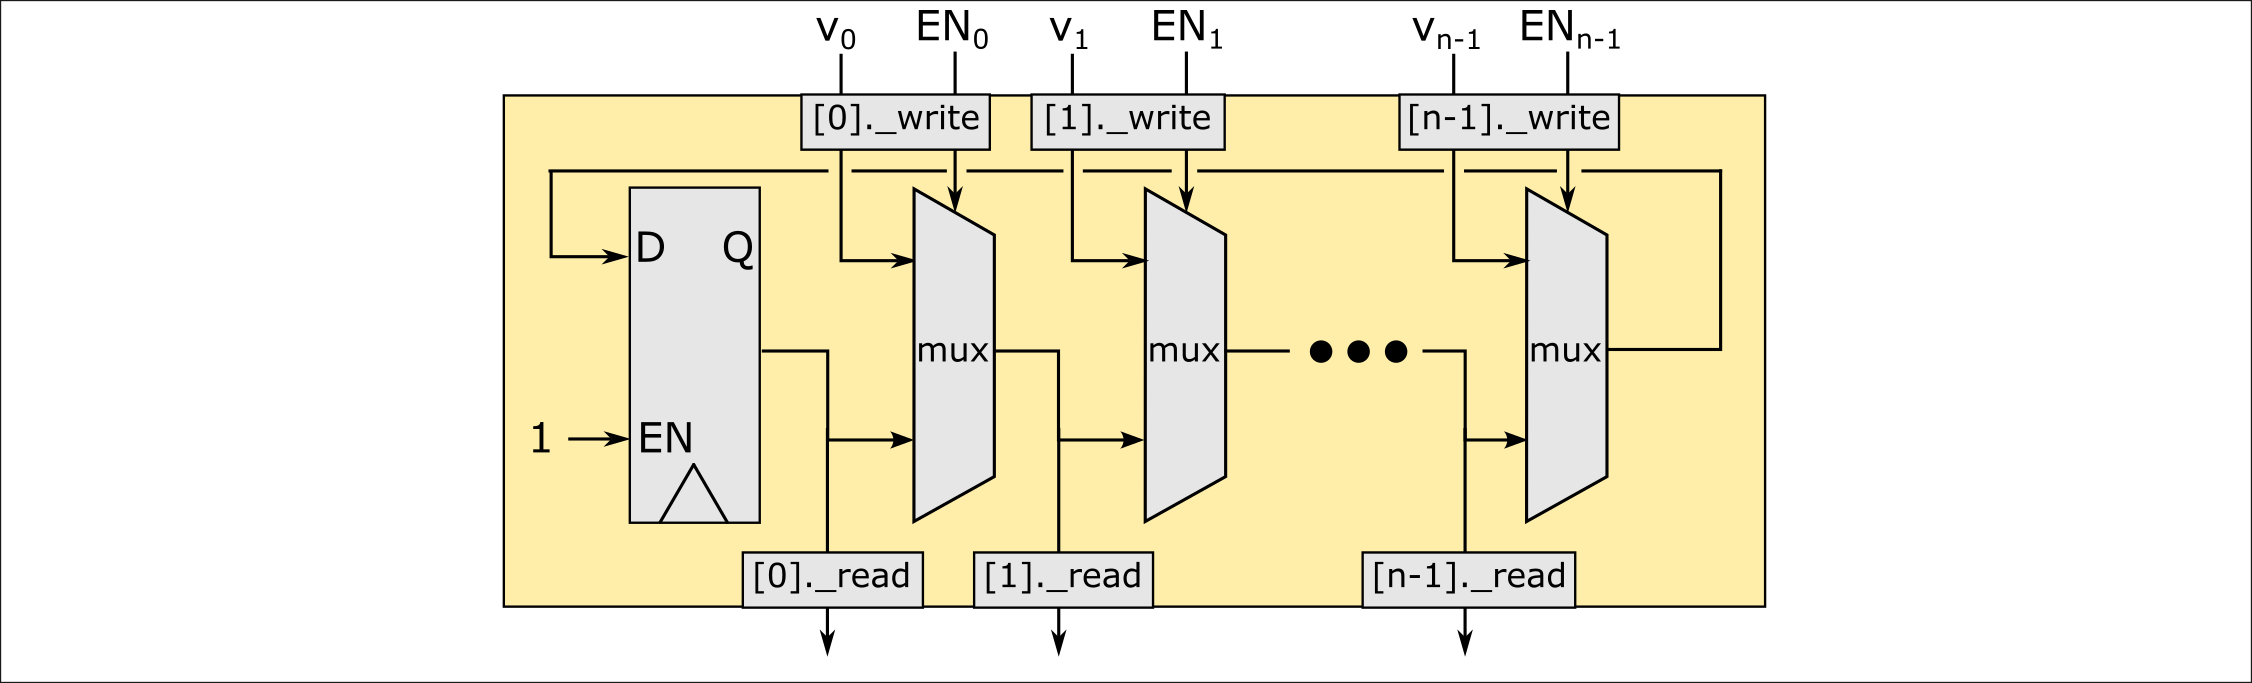
\includegraphics[width=6in,angle=0]{Figures/Fig_CReg_HW}}
  \caption{\label{Fig_CReg_HW} A possible hardware implementation of a CReg}
\end{figure}
On the left is a regular D flip flop.  To its right is a combinational
circuit comprised of a series of $n$ multiplexers, where $n$ is the
interface array size for the CReg.  The top and bottom depict the $n$
\verb|.write| and \verb|.read| methods, respectively.

The $j^{th}$ multiplexer selects either the output of the previous
element (D flip flop or multiplexer), or the data argument of the {\tt
[$j$].\_write} method.  The selection is controlled by the EN input of
the {\tt [$j$].\_write} method.  Thus, if the {\tt [$j$].\_write} method
is currently being invoked, that data is fed onward, otherwise the
data from the previous element.

The {\tt [$j$].\_read} method returns the value before the $j$'th
multiplexer.

A little study of the diagram will show that it indeed implements the
semantics described in the previous section.

% ================================================================

\subsection{A Faster Up-Down Counter, using a {\tt CReg}}

\label{Sec_Faster_Up_Down_Counter}

Here is an alternative module implementing our Up-Down Counter
interface, using a \verb|CReg|:

{\footnotesize
\begin{Verbatim}[frame=single, numbers=left]
module mkUp_Down_Counter_I (Up_Down_Counter_IFC);
   // STATE
   Array #(Reg #(Bit #(4))) crg_counter <- mkCReg (2,15);

   // ----------------------------------------------------------------
   // INTERFACE
   method Action incr (rg_counter != 15);
      rg_counter [0] <= rg_counter [0] + 1;
   endmethod

   method Action decr; (rg_counter != 0);
      rg_counter [1] <= rg_counter [1] - 1;
   endmethod

   method Bit #(4) val;
      return rg_counter [0];
   endmethod
endmodule
\end{Verbatim}
}

Now, three rules invoking the three methods can all be invoked on the
same clock.  Further, when they are invoked in the same clock, it
answers the question, ``What value does \verb|val| return?'':

\begin{quote}
The original value in the CReg? \\
Or the value after the increment? \\
Or the value after the decrement? \\
Or the value after the increment and decrement?
\end{quote}

Per the semantics of \verb|CReg|, it returns \verb|rg_counter[0]|,
which is the original value in the CReg.  If we were to return
\verb|rg_counter[1]|, it would return the value after the increment
and before the decrement.  If our CReg had an array of 3 register
interfaces intead of 2, we could return \verb|rg_counter[2]| which
would be the value after both the increment and decrement.

% ****************************************************************

\section{Example: Using a CReg for the RISC-V CSR {\tt mcycle}}

\label{Sec_CSR_mcycle}

One of the RISC-V CSRs is {\tt mcycle}.  This CSR is incremented by
the hardware automatically on every clock, to count total clock
cycles.  But this CSR can also be written from RISC-V code using a
CSRRxx instruction (which was described in Section~\ref{sec_CSRRxx}).
Suppose the CSR contains the value $n$, and we are executing a CSRRxx
instruction that wants to write $m$ to the CSR.  After the clock
instant, should the value be $n+1$? Or $m$? Or $m+1$? Or something
else?  The RISC-V specification says it should be $m$, the value
written by the CSRRxx instruction.

This can be cleanly expressed using a CReg.

{\footnotesize
\begin{Verbatim}[frame=single, numbers=left, label=from src\_Common/CSRs.bsv]
   Array #(Reg #(Bit #(64))) csr_mcycle <- mkCReg (2, 0);
\end{Verbatim}
}

The automatic increment in every cycle is performed by this rule in
the CSRs module:
{\footnotesize
\begin{Verbatim}[frame=single, numbers=left, label=from src\_Common/CSRs.bsv]
   rule rl_count_cycles;
      csr_mcycle [0] <= csr_mcycle [0] + 1;
   endrule
\end{Verbatim}
}

To execute a CSRRxx instruction, a rule in the CPU invokes a method in
the CSRs module which contains this code:

{\footnotesize
\begin{Verbatim}[frame=single, numbers=left, label=from src\_Common/CSRs.bsv]
   csr_mcycle [1] <= csr_val;
\end{Verbatim}
}

The use of the indexes [0] and [1] ensure that when a CSRRxx
instruction is executed, its value will override the incremented value
written by \verb|rl_count_cycles|.

% ****************************************************************

\section{PipelineFIFOs and BypassFIFOs}

\label{Sec_SpecialFIFOs}

Consider the following module implementing a 1-element FIFO with a
\verb|FIFOF| interface:

{\footnotesize
\begin{Verbatim}[frame=single, numbers=left]
module mkFIFOF (FIFOF #(Bit #(32)));
   Reg #(Bit #(32)) rg_data <- mkRegU;
   Reg #(Bool)      rg_full <- mkReg (False);

   // ----------------
   // INTERFACE

   method Bool notEmpty ();
      return rg_Full;
   endmethod

   method Bit #(32) first () if (rg_full);
      return rg_data;
   endmethod

   method Action deq () if (rg_full);
      rg_full <= False;
   endmethod

   method Bool notFull ();
      return (! rg_Full);
   endmethod

   method Action enq (Bit #(32) x) if (! rg_full);
      rg_data <= x;
      rg_full <= True;
   endmethod

   method Action clear;
      rg_full <= False;
   endmethod
endmodule
\end{Verbatim}
}

Consider a producer rule \verb|rl_P| that invokes \verb|enq|, and a
consumer rule \verb|rl_C| that invokes \verb|first| and \verb|deq|,
as shown in Figure~\ref{Fig_FIFO_Producer_Consumer}.
\begin{figure}[htbp]
  \centerline{
\includegraphics[width=6in,angle=0]{Figures/Fig_FIFO_Producer_Consumer}}
  \caption{\label{Fig_FIFO_Producer_Consumer}A producer and consumer connected with a FIFO}
\end{figure}

These rules cannot fire at the same instant (on the same clock)
because both of them read and write register \verb|fg_Full| (because
both \verb|enq| and \verb|deq| read and write the register).

Let us use a CReg to relax this constraint, in two different ways.

% ================================================================

\subsection{{\tt PipelineFIFOF}}

{\footnotesize
\begin{Verbatim}[frame=single, numbers=left]
module mkPipelineFIFOF (FIFOF #(Bit #(32)))
   Reg #(Bit #(t))     rg_data  <- mkRegU;
   Array #(Reg #(Bool)) crg_full <- mkCReg (3, False);

   // ----------------
   // INTERFACE

   method Bool notEmpty ();
      return crg_Full [0];
   endmethod

   method Bit #(32) first () if (crg_Full [0]);
      return rg_data;
   endmethod

   method Action deq () if (crg_Full [0]);
      crg_Full [0] <= False;
   endmethod

   method Bool notFull ();
      return (! crg_Full [1]);
   endmethod

   method Action enq (Bit #(32) x) if (! crg_Full [1]);
      rg_data      <= x;
      crg_Full [1] <= True;
   endmethod

   method Action clear;
      crg_Full [2] <= False;
   endmethod
endmodule
\end{Verbatim}
}

Again, consider a producer rule \verb|rl_P| that invokes \verb|enq|,
and a consumer rule \verb|rl_C| that invokes \verb|first| and
\verb|deq|.  Now, these rules \emph{can} fire together at the same
instant (on the same clock).

Because of the choice of indexes we can see that, in the equivalent
rule-at-a-time semantics, \verb|rl_C| fires \emph{before} \verb|rl_P|.
Thus, even if the FIFO was full at the start of the clock, \verb|rl_P|
can still \verb|enq| into the FIFO, \emph{provided} \verb|rl_C| is
firing on the same clock.  Per the rule-at-a-time semantics,
\verb|rl_C| fires first, which empties the FIFO, {\ie} \verb|rl_P|
sees the FIFO as empty and is therefore able to \verb|enq| into it.

As a separate observation, we can see that another rule invoking
\verb|clear|, too, can fire on the same clock as \verb|rl_P| and
\verb|rl_C| and, because of its index, logically fires ``last'', and
so will leave the FIFO in a finally empty state.

If we examine the Verilog generated for \verb|mkPipelineFIFOF|, we
will see that the READY signal for \verb|enq| incorporates the ENABLE
signal of the \verb|deq| method (because, if the FIFO is full at the
previous clock, in this clock \verb|enq| can only be invoked if
\verb|deq| is also being invoked).  Thus, there is a
\emph{combinational path} backward through the FIFO (a path that only
involves wires and gates and no state-element) from the \verb|deq|
method to the \verb|enq| method.  This is illustrated in
Figure~\ref{Fig_Combo_path_in_mkPipelineFIFOF}.
\begin{figure}[htbp]
  \centerline{\includegraphics[width=6in,angle=0]{Figures/Fig_Combo_path_in_mkPipelineFIFOF}}
  \caption{\label{Fig_Combo_path_in_mkPipelineFIFOF}
           Combinational path through {\tt mkPipelineFIFOF}}
\end{figure}

This kind of FIFO is called a ``Pipeline FIFO'' because it is an ideal
candidate for the FIFO between stages of a pipeline.  It allows the
downstreanm stage (the consumer) and the upstream stage (the producer)
to fire on the same clock, advancing data in a piplined manner.  It is
so useful that it is available in the \emph{bsc} library in the
\verb|SpecialFIFOs| package.

% ================================================================

\subsection{{\tt BypassFIFOF}}

In this version, we change the CReg indexes used by the methods.

{\footnotesize
\begin{Verbatim}[frame=single, numbers=left]
module mkPipelineFIFOF (FIFOF #(Bit #(32)));
   Array #(Reg #(Bit #(32))) crg_data <- mkCRegU (2);
   Array #(Reg #(Bool))      crg_full <- mkCReg (3, False);

   // ----------------
   // INTERFACE

   method Bool notEmpty ();
      return crg_Full [1];
   endmethod

   method Bit #(32) first () if (crg_Full [1]);
      return crg_data [1];
   endmethod

   method Action deq () if (crg_Full [1]);
      crg_Full [1] <= False;
   endmethod

   method Bool notFull ();
      return (! crg_Full [0]);
   endmethod

   method Action enq (Bit #(32) x) if (! crg_Full [0]);
      crg_data [0] <= x;
      crg_Full [0] <= True;
   endmethod

   method Action clear;
      crg_Full [0] <= False;
   endmethod
endmodule
\end{Verbatim}
}

Again, consider a producer rule \verb|rl_P| that invokes \verb|enq|,
and a consumer rule \verb|rl_C| that invokes \verb|first| and
\verb|deq|.  These rules \emph{can} fire together at the same instant
(on the same clock).

Because of the choice of indexes we can see that, in the equivalent
rule-at-a-time semantics, \verb|rl_P| fires \emph{before} \verb|rl_C|.
Thus, even if the FIFO was empty at the start of the clock,
\verb|rl_C| can still read \verb|first|, and \verb|deq| the FIFO,
\emph{provided} \verb|rl_P| is firing on the same clock.  Per the
rule-at-a-time semantics, \verb|rl_P| fires first, which fills the
FIFO, {\ie} \verb|rl_C| sees the FIFO as full and is therefore able to
use \verb|first| and \verb|deq|.

As a separate observation, we can see that another rule invoking
\verb|clear|, too, can fire on the same clock as \verb|rl_P| and
\verb|rl_C| and, because of its index, logically fires ``last'', and
so will leave the FIFO in a finally empty state.

If we examine the Verilog generated for \verb|mkBypassFIFOF|, we will
see that the READY signal for \verb|first| and \verb|deq| incorporates
the ENABLE signal of the \verb|enq| method (because, if the FIFO is
empty at the previous clock, in this clock \verb|first| and \verb|deq|
can only be invoked if \verb|enq| is also being invoked).  Further,
when \verb|enq| and \verb|first| are invoked in the same clock, the
data argument to \verb|enq| is passed straight though to the data
result of \verb|first|.  Thus, there are several \emph{combinational
paths} forward through the FIFO (paths that only involve wires and
gates and no state-element) from the \verb|enq| method to the
\verb|first| and \verb|deq| methods.
This is illustrated in
Figure~\ref{Fig_Combo_path_in_mkBypassFIFOF}.
\begin{figure}[htbp]
  \centerline{\includegraphics[width=6in,angle=0]{Figures/Fig_Combo_path_in_mkBypassFIFOF}}
  \caption{\label{Fig_Combo_path_in_mkBypassFIFOF}
           Combinational paths through {\tt mkBypassFIFOF}}
\end{figure}

This kind of FIFO is called a ``Bypass FIFO'' because of the way data
can ``bypass'' the FIFO from \verb|enq| to \verb|first|.  It is so
useful that it is available in the \emph{bsc} library in the
\verb|SpecialFIFOs| package.

% ================================================================

\subsection{Back-to-back compositions of {\tt BypassFIFOF} and {\tt PipelineFIFOF}}

\label{Sec_mkBypassFIFOF_mkPipelineFIFOF}

An interesting component is a back-to-back composition of the two
FIFOs discussed in the previous sections.  Consider this code
fragment:

{\footnotesize
\begin{Verbatim}[frame=single, numbers=left]
module mk... (...);
   FIFOF #(Bit #(32)) f_bypass   <- mkBypassFIFOF;
   FIFOF #(Bit #(32)) f_pipeline <- mkPipelineFIFOF;

   // Producer rule (into f_bypass's enq side)
   rule rl_P;
      ... f_bypass.enq (x);
   endrule

   // Connect f_bypass's first/deq side to to f_pipeline's enq side
   mkConnection (to_FIFO_O (f_bypass), to_FIFO_I (f_pipeline));

   // Consumer rule (from f_pipeline's first/deq side)
   rule rl_C;
      let y = f_pipeline.first;
      f_pipeline.deq;
   endrule
endmodule
\end{Verbatim}
}

This is illustrated in Figure~\ref{Fig_Composed_FIFO_Producer_Consumer}.
\begin{figure}[htbp]
  \centerline{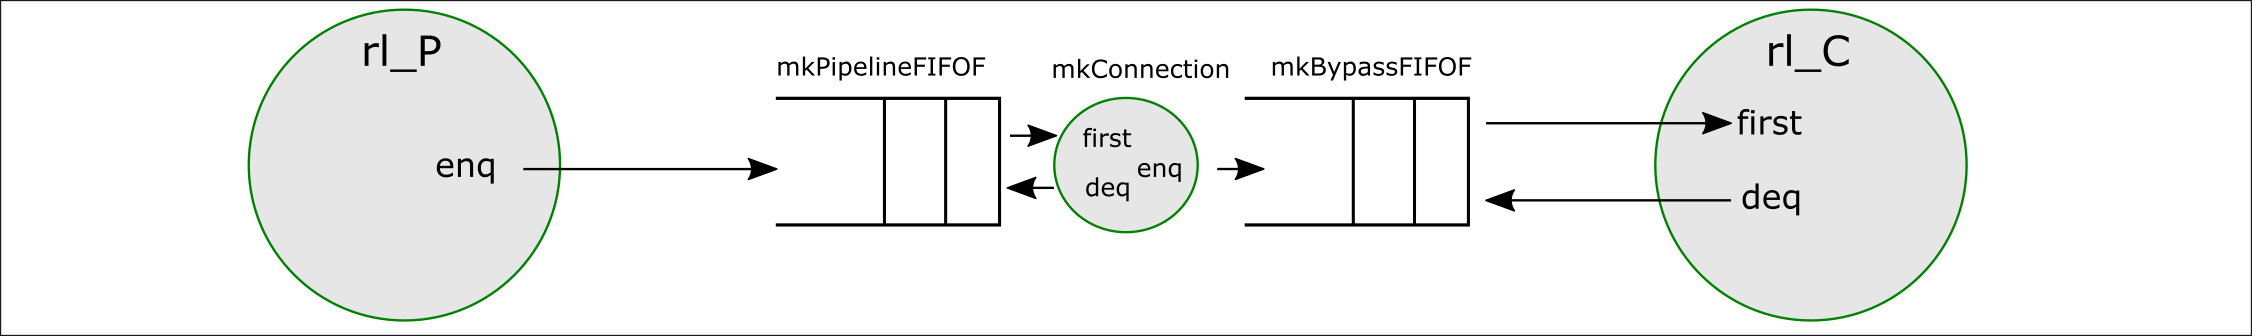
\includegraphics[width=6in,angle=0]{Figures/Fig_Composed_FIFO_Producer_Consumer}}
  \caption{\label{Fig_Composed_FIFO_Producer_Consumer}
                  A producer and consumer connected with a composed BypassFIFO-PipelineFIFO.}
\end{figure}
This composition has some pleasant properties:

\begin{itemize}

 \item Normally, if we connect two FIFOs back-to-back like this, it
       will always take a minimum of two ticks for a datum to traverse
       through (from \verb|enq| to \verb|first|/\verb|deq|---one tick
       in the first FIFO and one tick in the second.  With this
       composition on the other hand, because of the Bypass FIFO, it
       can traverse in a single tick.

 \item Like the ordinary \emph{bsc} library \verb|mkFIFOF|, and unlike
       \verb|mkPipelineFIFOF| and \verb|mkBypassFIFOF| by themselves,
       the producer rule \verb|rl_P| side and the consumer rule
       \verb|rl_C| have no ordering constraints (they are conflict
       free).  They can fire in the same clock and can go in either
       logical order.

 \item There are no combinational paths through the pair of FIFOs!
       One can verify this by generating the Verilog for the composed
       FIFOs and analyzing it (which, fortunately, does not have to be
       done by hand, because when the \emph{bsc} compiler generates
       Verilog for a module, it helpfully reports combinational paths,
       if any, through the module.

\end{itemize}

These properties make it very attractive to use this composition to
connect stages in a pipeline, enabling a \emph{modular} separation of
stages.  We can place \verb|mkBypassFIFOF| in the module for the
upstream stage, place \verb|mkPipelineFIFOF| in the module for the
downstream stage, and connect them in the parent module with
\verb|mkConnection|.
This is illustrated in Figure~\ref{Fig_Composed_FIFO_modularity}.
\begin{figure}[htbp]
  \centerline{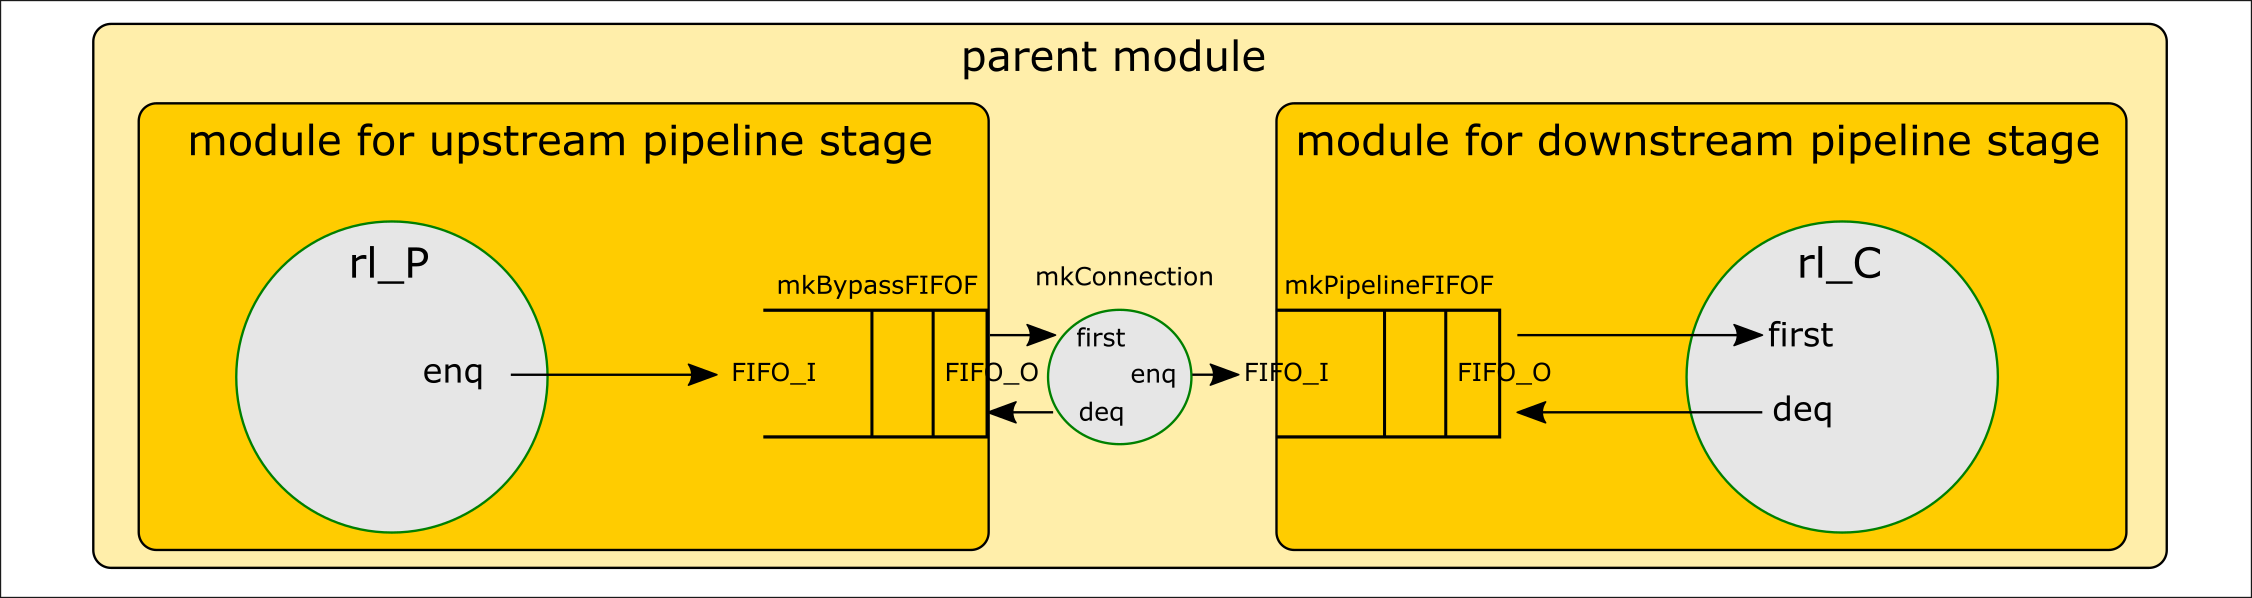
\includegraphics[width=6in,angle=0]{Figures/Fig_Composed_FIFO_modularity}}
  \caption{\label{Fig_Composed_FIFO_modularity}
                  Pipeline-stage modularity enabled by composing a BypassFIFO and a PipelineFIFO}
\end{figure}
We use this structure extensively and exclusively in Fife to connect
its stages.

The only downside is that the composition has two data registers, one
each in \verb|mkBypassFIFOF| and \verb|mkPipelineFIFOF|.  In many
applications, this does not matter much, {\ie} the overall state size
is dominated by other components, and this addition is in the noise.

% ----------------
\Exercise

What happens if we reverse the composition---use
\verb|mkPipelineFIFOF| upstream and \verb|mkBypassFIFOF| downstream?

\begin{itemize}

 \item How many ticks will it take for a datum to traverse the pair?

 \item Will \verb|rl_P| and \verb|rl_C| still be conflict-free (and
       therefore can fire in either logical order)?

 \item Are there any combinational paths through the pair?

 \item Consider combinational paths in rule \verb|rl_P| ending at the
       \verb|enq| method of the first FIFO, and combinational paths in
       rule \verb|rl_C| starting at the \verb|first| method of the
       second FIFO.  What is the difference between these when we
       compose \verb|mkBypassFIFOF| $\longrightarrow$ \verb|mkPipelineFIFOF|
       {\vs} \verb|mkPipelineFIFOF| $\longrightarrow$ \verb|mkBypassFIFOF|?

\end{itemize}

\Endexercise

% ****************************************************************

\section{Alternatives to CRegs: RWires and their variants (deprecated)}

\label{Sec_RWires}

In digital hardware,

\begin{itemize}

 \item a register communicates a value across clocks (from one clock to succeeding clocks), and

 \item a wire communicates a value within a clock (from state element
       to gate, from gate to gate, and from gate to state element).

\end{itemize}

A BSV register is a standard digital hardware register.  A BSV CReg
plays the role of both register and wires, communicating values
flexibly within a clock and across clocks, depending on whether its
methods are invoked within a clock or across clocks.  The concept of
CRegs was first proposed by Daniel Rosenband and Arvind at MIT
\cite{RosenbandMEMOCODE04, Rosenband2005b} (they were originally
called ``Ephemeral History Registers'' or EHRs).

Before the invention of CRegs, BSV had a facility to manage
intra-clock communication, called the ``\verb|RWire|''.  These are
still available in BSV, along with several specializations:
``\verb|Wire|'', ``\verb|BypassWire|'', ``\verb|DWire|'', and
``\verb|PulseWire|''.  Please see the \emph{bsc} library documentation
for detailed information.

CRegs are semantically preferable to RWires because they fit cleanly
into rule-at-a-time semantics, where a CReg can be treated as an
ordinary register.  The semantics of a BSV program with CRegs can be
explained purely at the rule-at-a-time level, with no mention of
clocks.  RWires, on the other hand, are only meaninful with clocks,
and are therefore semantically messier.

Since the inclusion of CRegs into the \emph{bsc} library, the need for
\verb|RWire| and its variants has mostly disappeared.

% ****************************************************************
